\chapter{\Large $HM\_QCv$: A Computationally Efficient Hybrid Model for Enhancing Quality Clusters in Visualization}


The $HM\_QCv$ approach is designed to preserve both (i) cluster information and (ii) local and global structures of high-dimensional data in visualization.  By leveraging UMAP \cite{umap_reference} and LaptSNE \cite{sun2023laplacian}, our approach ensures computational efficiency and significantly reduces processing time compared to LAPtSNE \cite{sun2023laplacian}.

The existing methodology LAPtSNE \cite{sun2023laplacian}, relies on the t-SNE \cite{tsne} method to compute the distance between the data objects, which is computationally intensive.  To address this limitation, we adopted UMAP \cite{umap_reference} in our proposed approach.  Before adopting UMAP \cite{umap_reference}, we conducted experiments on three benchmark datasets to evaluate both the t-SNE \cite{tsne} and UMAP \cite{umap_reference} approaches, measuring their processing times as presented in Table \ref{tsneumapcmp} in Section 4.2. The results clearly demonstrate that UMAP \cite{umap_reference} is more computationally efficient than t-SNE \cite{tsne}. Hence, our approach, $HM\_QCv$, is more computationally efficient than LAPtSNE \cite{sun2023laplacian} while ensuring both local and global structure by preserving high-quality cluster visualization, offering promising practical implications for the field of data visualization.



\subsection{Leveraging combined approaches}

One approach for addressing the research questions outlined in Section 1 is to leverage the strengths of UMAP \cite{umap_reference} and LAPtSNE \cite{sun2023laplacian} while integrating their partial components to develop more comprehensive solutions. This combined method may reveal insights that would be unattainable with either technique used independently. Table \ref{rqofpm} presents a comparative analysis of the characteristics by the proposed model $HM\_QCv$ and existing NLDR techniques.



\begin{table}[!htbp]
 \caption{A comparative analysis of Proposed Model and Existing Techniques}
    \centering
   \resizebox{0.98\textwidth}{!}{
    \begin{tabular}{|c|c|c|c|c|}
        \hline
       \textbf{ \diagbox[innerwidth = 6.3cm]{Technique}{Characteristics}} & \textbf{Computationally efficient} &  \textbf{Quality cluster visualization} & \textbf{Local Structure} & \textbf{Global Structure} \\
         \hhline{~|-|-|-|-|}
        & \textbf{(RQ1)} &  \textbf{(RQ2)} &  \textbf{(RQ3)} & \textbf{(RQ3)} \\
        \hhline{-|-|-|-|-|}
         t-SNE \cite{tsne} & \xmark  &  \xmark &  \cmark  & \textbf{Partially retains}\\
          \hline
        UMAP \cite{umap_reference} &  \cmark  & \xmark & \textbf{Partially retains} &  \cmark \\
         \hline
         LAPtSNE \cite{sun2023laplacian} &  \xmark &  \cmark &  \cmark &  \cmark \\
        \hline
         $\bm{HM\_QCv}$ \textbf{(Proposed approach)} &  \cmark &  \cmark &  \cmark &  \cmark\\
        \hline
    \end{tabular}
   }
    \label{rqofpm}
\end{table}

Traditional techniques \cite{tsne} \cite{umap_reference} \cite{sun2023laplacian} exist for visualizing high-dimensional data. Still, they face limitations by covering all characteristics, such as (i) minimizing computational costs, (ii) providing high-quality cluster visualizations, and (iii) preserving both local and global structures. Local structures refer to the relationships between nearby data points \cite{tsne}, whereas global structures encompass the overall distribution of the data \cite{umap_reference} \cite{tenenbaum2000global}.   

Sun et al. \cite{sun2023laplacian} developed an approach that uses the t-SNE \cite{tsne} methodology to preserve the local and global structure and incorporates a symmetric Laplacian matrix, the regularization technique for cluster quality when visualizing the data. However, this approach, while improving the representation of clusters, also increases the computational complexity due to t-SNE \cite{tsne}.

%Sun et al. \cite{sun2023laplacian} developed an approach that uses the t-SNE \cite{tsne} methodology to preserve the local structure by incorporating a symmetric Laplacian matrix, the regularization technique. This technique has the potential to greatly enhance cluster quality when visualizing the data. However, this approach, while improving the representation of clusters, also increases the computational complexity due to t-SNE \cite{tsne}.

One effective way to address the computational overhead of t-SNE \cite{tsne} is to leverage the strengths of UMAP \cite{umap_reference}. Additionally, UMAP \cite{umap_reference} has the characteristics to preserve the global structure, and therefore, leveraging the regularization technique of LAPtSNE \cite{sun2023laplacian} with UMAP methodology will further improve the quality of cluster visualization. Hence, an $HM\_QCv$ approach is proposed.



 
\subsubsection{Mathematical Derivation of the Proposed Model}

The cross-entropy loss is minimized between the high and low-dimensional probabilities ($\min_{Z} \text{CrossEntropy}(HDP_{ij}, LDP_{ij})$) and is equivalent to the gradient of cross-entropy loss ($\nabla \mathcal{L}_{CE}(Z)$).  

The cluster information is obtained in the proposed model using a symmetric graph laplacian matrix. The desired clusters \textit{`NC'} are preserved using ($\lambda \text{Tr}(EV_{LP_{ld}} LP_{ld} EV_{LP_{ld}}^T)$) is equivalent to the gradient of regularization ($\lambda \nabla \mathcal{L}_{Reg}(Z)$). Chung et al. \cite{chung1997spectral} have stated that the multiplicity of \textit{`NC'} of the eigenvalue zero of a Laplacian matrix (L) corresponds to \textit{`NC'} distinct clusters. Therefore, an effort is made to maximize the number of eigenvalues in (L) to enhance the number of clusters in a low-dimensional space.


The proposed model is as follows
\begin{equation}
    \min_{Z} \text{CrossEntropy}(HDP_{ij} , LDP_{ij}) + \lambda \text{Tr}(EV_{LP_{ld}} LP_{ld} EV_{LP_{ld}}^T) 
\end{equation}

\begin{itemize}
    \item $EV_{LP_{ld}}$ represents the eigenvectors of the Laplacian matrix ($LP_{ld}$) with the fewest \textit{`NC'} eigenvalues produced from a low-dimensional affinity matrix $LD_{af}$.
    \item $HDP_{ij}$ represents symmetric high-dimensional probabilities, whereas $LDP_{ij}$ represents low-dimensional probabilities.
    \item The regularization term $\lambda \text{Tr}(EV_{LP_{ld}} LP_{ld} EV_{LP_{ld}}^T)$ maximizes the number of zero eigenvalues in the Laplacian matrix $LP_{ld}$, acting as repulsive forces to maintain separation between distinct points corresponding to the \textit{`NC'} clusters in high-dimensional space.
\end{itemize}



The proposed model constructs the k-nearest neighbour graph using \\UMAP \cite{umap_reference} and obtains the desired clusters through LAPtSNE \cite{sun2023laplacian}, utilizing the symmetric graph laplacian matrix, which is represented using the below equation:

\begin{equation}
    \nabla \mathcal{L}_{CE}(Z) + \lambda \nabla \mathcal{L}_{Reg}(Z))
\end{equation}


Therefore, our proposed approach achieves greater computational efficiency by leveraging the strength of partial component UMAP \cite{umap_reference} and is robust to outliers. Our approach ensures the formation of high-quality clusters through the strengths of partial component LAPtSNE \cite{sun2023laplacian} by preserving both the local and global structure of the data. While leveraging the combined approach, our approach is also prominently proved by experiments that it enhances the efficacy of cluster visualization within low-dimensional space.



\begin{algorithm}[!h]
\footnotesize
\KwIn{Dataset $A \in \mathbb{R}^{N \times D}$, target dimension $d$, number of clusters $NC$, tuning (regularization) parameter $\lambda$, number of nearest neighbours $k$, learning rate $\alpha$, maximum iterations $IT$}%($0.001$ to $1$),  % ($10^{-6}$ to $1$)}
\KwOut{Low-dimensional embedding $Z_{IT} \in \mathbb{R}^{N \times d}$}

Construct the $k$-nearest neighbour (k-NN) graph $G = (V, E, w)$ from $A$

$HDP_{ij} \leftarrow \exp \left( - \frac{\max(0, d(x_i, x_j) - \rho_i)}{\sigma_i} \right)$ \Comment{Compute High-Dimensional Probabilities $HDP_{ij}$}

Represent the $HDP_{ij}$ as affinity matrix $HD_{af}$

Symmetrize the affinity matrix $SHD_{af} = \frac{HD_{af} + {HD_{af}}^T}{2}$

Compute the Laplacian matrix $LP_{hd}$ from the symmetrized affinity matrix $SHD_{af}$. 

Initialize the low-dimensional embedding $Z_0$ by selecting the top $d$ eigenvectors of the Laplacian $LP_{hd}$ as given below $Z_0 \leftarrow [EV_1(LP_{hd}), \dots, EV_d(LP_{hd})]$. 

\For{$t = 1$ \textbf{to} $IT$}{
   $LDP_{ij} \leftarrow \left( 1 + a \frac{\| y_i - y_j \|^2}{2b} \right)^{-1}$ \Comment{Compute Low-Dimensional Probabilities $LDP_{ij}$}
    
    Represent the $LDP_{ij}$ as affinity matrix $LD_{af}$

    Compute the Laplacian matrix $LP_{ld}$ from $LD_{af}$

    Compute gradient of cross-entropy loss $\nabla \mathcal{L}_{CE}(Z)$ between $\{HDP_{ij}\}$ and $\{LDP_{ij}\}$ \Comment{$Z \leftarrow Z_{t}$}

    Compute gradient of regularization $\nabla \mathcal{L}_{Reg}(Z)$ using Laplacian matrix $LP_{ld}$
    
    Update $Z_t \leftarrow Z_{t-1} - \alpha \left( \nabla \mathcal{L}_{CE}(Z) + \lambda \nabla \mathcal{L}_{Reg}(Z) \right)$.
}


\caption{\footnotesize{Hybrid Model for Quality Cluster Visualization ($\bm{HM\_QCv}$)}}
\end{algorithm}






\subsection{Phases of HM\_QCv approach}


The proposed framework of the Hybrid Model for Quality Cluster Visualization shown in \textbf{Figure \ref{hmqcv}} is divided into four crucial phases, which are discussed below, and the details are provided in subsequent subsections.


\begin{itemize}

\item Construct k-nearest neighbour graph for High-Dimensional Data and determine its Probabilities.

\item Construction of the Laplacian Matrix for k-nearest neighbour graph.

\item Determine Low-Dimensional Probabilities and Construct the Corresponding Laplacian Matrix. 

\item Optimize Low-Dimensional Embeddings through Gradient Computation of Cross-Entropy Loss and Regularization. 
\end{itemize}

\begin{figure}[!htbp]
    \centering
    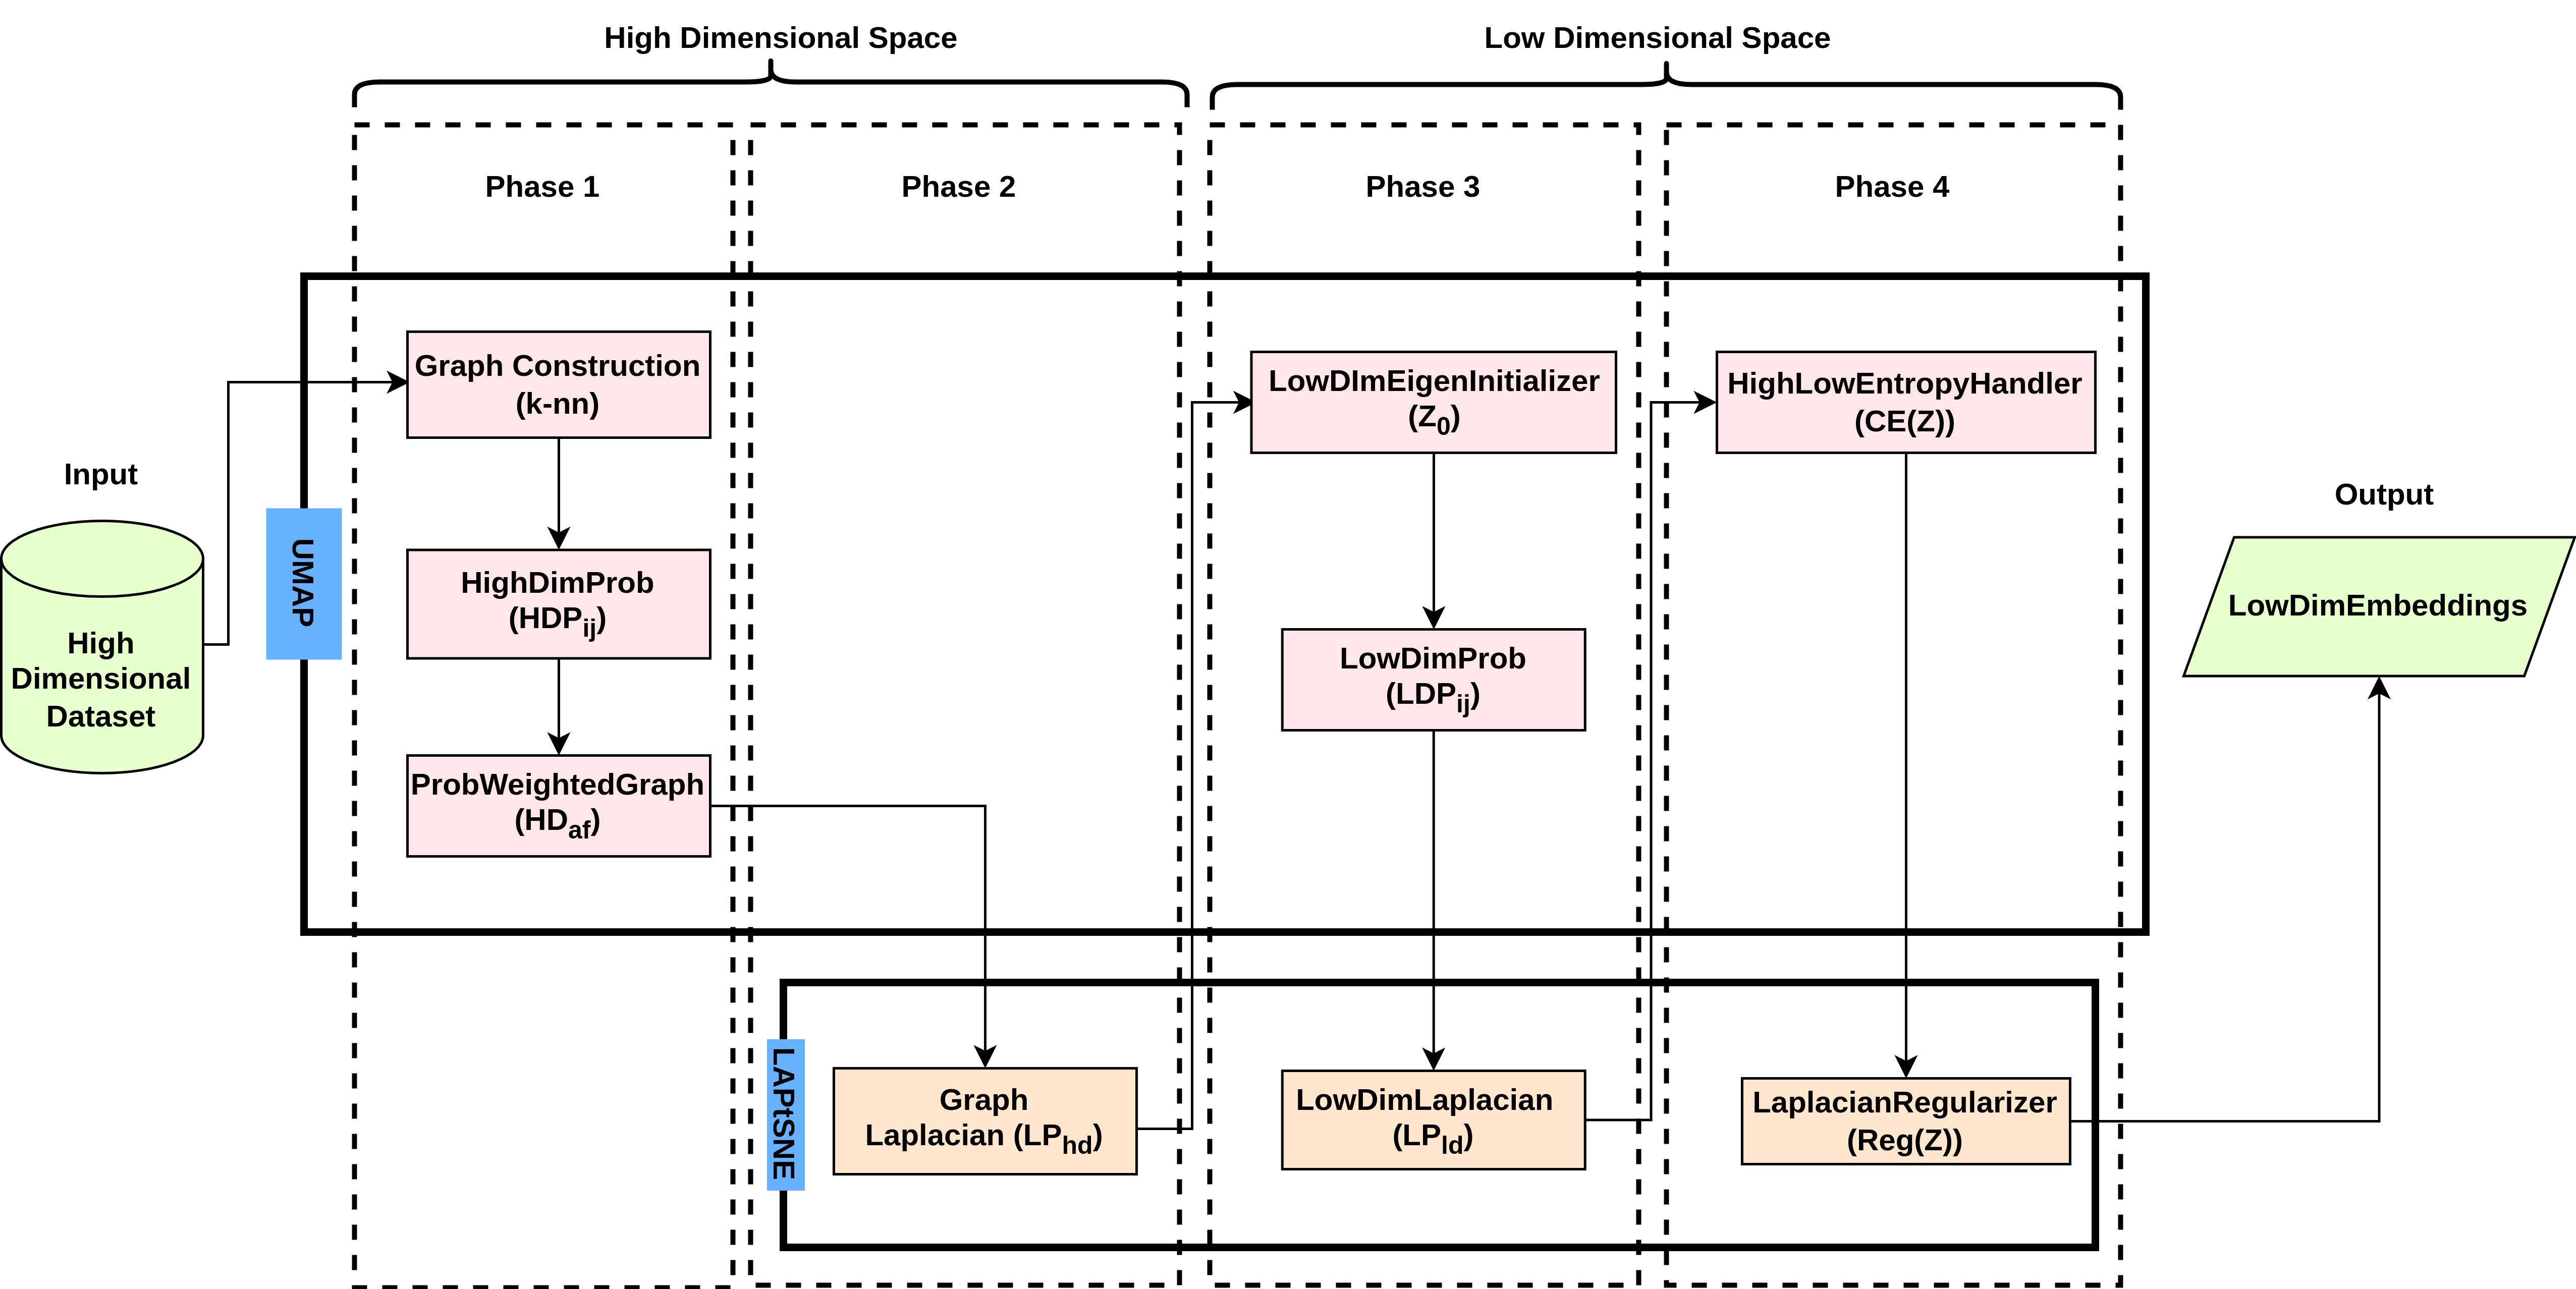
\includegraphics[width = \textwidth]{HMQCvImages/HybridModelQualityCluster-Page-3.drawio (1).png}  
    \caption{Proposed Framework of Hybrid Model for Quality Cluster Visualization}
    \label{hmqcv}
\end{figure}

\subsubsection{Graph Construction for High-Dimensional Data and determine its Probabilities}
High-dimensional data ($\mathbb{R}^{N \times D}$) is taken as input for the Phase 1.

Phase 1 involves three components:




\begin{enumerate}[label=\roman*]
    \item \textbf{ Graph Construction} component determines the k-nearest neighbours for each data point $x_i$ in high-dimensional space by calculating the pairwise distances using the Euclidean distance metric.
    
    \item \textbf{HighDimProb} component computes the high-dimensional  probabilities using parameters $\rho_i$ and $\sigma_i$ which are determined  using the equation \ref{equ3}. $\rho_i$ signifies the distance from a data point to the  nearest neighbour, and $\sigma_i$ represents the normalizing factor \cite{umap_reference}.
    \begin{equation}\label{equ3}
      \sum_{j=1}^{k} \exp\left( \sigma_i - \max(0, d(x_i, x_{ij}) - \rho_i) \right) = \log_2(k)  
    \end{equation}
    For each data point $x_i$, $\sigma_i$ is computed such that the sum of the high-dimensional probabilities across its k-nearest neighbours equals $\log_2(k)$. High-dimensional probabilities ($HDP_{ij}$) are calculated \cite{umap_reference} using equation (4).
    \begin{equation}
        HDP_{ij} = \exp\left( -\frac{\max(0, d(x_i, x_{ij}) - \rho_i)}{\sigma_i} \right)
    \end{equation}

    \item \textbf{ProbWeightedGraph} component is the weighted k-nearest neighbour graph, denoted as $w_knn_g=(V,E,w)$, is constructed using the k-nearest neighbour graph and high-dimensional probabilities ($HDP_{ij}$), where $V$ represents the data points, $E$ is the edges connecting to the k-nearest neighbours, and $w$ corresponds to $HDP_{ij}$. The $HDP_{ij}$ are represented by the affinity matrix $HD_{af}$.    

\end{enumerate}

%%
Symmetrizing $HD_{af}$ of the Phase 1 component before proceeding to Phase 2 computations. The $HD_{af}$ is asymmetric due to the nature of the k-nearest neighbour graph. In this graph, k-nearest neighbour relationships may not be mutual; i.e., if point $x_i$ is one of the k-nearest neighbours of points $x_j$, it does not necessarily imply that $x_j$ is the k-nearest neighbour of $x_i$. The Affinity matrix $HD_{af}$ is symmetrized \cite{umap_reference} using equation (5) and is considered as $SHD_{af}$.

    \begin{equation}
         SHD_{af} = \frac{HD_{af} + {HD_{af}}^T}{2}
    \end{equation}

\subsubsection{Construction of the Laplacian Matrix}
In Phase 2 \textbf{ GraphLaplacian} component uses the Laplacian matrix, which can reveal the number of clusters in the data, with the multiplicity \textit{`k'} of the zero eigenvalues corresponding to the number of clusters. Sun et al. \cite{sun2023laplacian} proposed maximizing the number of zero eigenvalues in the Laplacian matrix to extract clusters from the data.

Hence, the strategy of Sun et al. \cite{sun2023laplacian} is adopted to use the Laplacian matrix in our proposed approach. The Laplacian matrix $LP_{hd}$ is calculated using the below equation (6). 

\begin{equation}
    LP_{hd} = I - D^{\frac{-1}{2}} (SHD_{af}) D^{\frac{-1}{2}} 
\end{equation}
    D is the degree matrix (a diagonal matrix) of $SHD_{af}$ defined as $D_{ii} = \sum_{j} {SHD_{af}}_{ij}$


\subsubsection{Determine Low-Dimensional Probabilities and Construct the Corresponding Laplacian Matrix}

Phase 3 adopts two methods and involves with three components which are discussed below. 
\begin{enumerate}
    \item Computing the Low-Dimensional probabilities using UMAP \cite{umap_reference} and further \item Constructing the Laplacian matrix in the Low-Dimensional space using \hspace{1cm} LAPtSNE \cite{sun2023laplacian}
\end{enumerate}
\begin{enumerate}[label=\roman*]
    \item \textbf{LowDimEigenInitializer} component initializes the low-dimensional space ($Z_{0}$) with eigenvectors (EV1....$EV_{d}$) of Laplacian $LP_{hd}$ shown in equation (6).
    
    \item \textbf{LowDimProb} component calculates the low-dimensional probabilities ($LDP_{ij}$) using equation (7).
    \begin{equation}
     LDP_{ij} = \left(1 + \frac{a||y_i - y_j||^2}{2b} \right)^{-1} 
    \end{equation}
    Here, \textit{`a'} is the scaling parameter, which regulates the effect of distance in the low-dimensional space, while \textit{`b'} is the decay rate, indicating how rapidly the probability decreases as the distance increases. These parameters are crucial in shaping the distribution of points in the low-dimensional space, thereby affecting the overall structure and clustering.\\
    The Low-dimensional probabilities $LDP_{ij}$ are represented as affinity matrix $LD_{af}$
    
    \item \textbf{LowDimLaplacian} component computes the the Laplacian matrix $LP_{ld}$ using equation (8).
    \begin{equation}
    LP_{ld} = I - D^{\frac{-1}{2}} (LD_{af}) D^{\frac{-1}{2}} 
    \end{equation}
    D is the degree matrix (a diagonal matrix) of LD\_{af} defined as $D_{ii} = \sum_{j} {LD_{af}}_{ij}$
    
    
\end{enumerate}


\subsubsection{Optimize Low-Dimensional Embeddings}    
Phase 4 employs two methods and involves with two components which are discussed below. 
\begin{enumerate}
    \item Minimizing the cross entropy between high and low-dimensional probabilities using UMAP \cite{umap_reference} and 
    \item Regularization using LAPtSNE \cite{sun2023laplacian}
\end{enumerate}

\begin{enumerate}[label=\roman*]
    \item \textbf{HighLowEntropyHandler} component minimizes the Cross-Entropy loss \cite{goodfellow2016deep} is minimized using equation (9) to preserve the clusters. 
    \begin{equation}
\begin{split}
    \min_{Z} \text{CrossEntropy}(HDP_{ij}, LDP_{ij}) \\
    \text{subject to} \quad \sum_{i=1}^{N} \bm{1}(\mu_i (LP_{ld}) = 0) = NC
\end{split}
\end{equation}

  
    In Laplacian matrix $LP_{ld}$, the $i^{th}$ eigenvalue of the matrix is denoted as \( \bm{\mu}(\cdot)\). The function \( \bm{1}(\cdot)\) serves as an indicator function returning 1 when the condition is satisfied and 0 otherwise. The objective of this formulation is to identify \textit{`NC'} clusters in Low-Dimesional space. 

    \item \textbf{LaplacianRegularizer} component obtains \textit{`NC'} desired clusters, the final equation after convergence as per \cite{sun2023laplacian}, is shown in equation (1).




\end{enumerate}
The output of the proposed framework of  Hybrid Model for Quality Cluster Visualization is derived finally by updating the embeddings in each iteration (\textit{t}) using the below equation (10)

\begin{equation}
    Z_t \leftarrow Z_{t-1} - \alpha \left( \nabla \mathcal{L}_{CE}(Z) + \lambda \nabla \mathcal{L}_{Reg}(Z) \right)
\end{equation}

$\alpha$ is the learning rate and $\lambda$ is the tuning (regularization) parameter.
The final Low-dimensional embedding after maximum iterations (IT) is $Z_{IT} \in \mathbb{R}^{N \times d}$.


We propose ($HM\_QCv$) an algorithm that integrates the strengths of existing strategies \cite{tsne} \cite{umap_reference} \cite{sun2023laplacian} into a unified approach. Finally, we provided outcomes to the research questions presented in Section 1.


\section{Results and Analysis}
The proposed ($HM\_QCv$) approach and existing NLDR approaches t-SNE \cite{tsne}, UMAP \cite{umap_reference}, and LAPtSNE \cite{sun2023laplacian} are experimented with the following supervised benchmark datasets.

To evaluate our methodology and assess its performance, we conducted experiments using supervised datasets where the number of clusters, denoted by \textit{`NC'}, aligns with the ground truth classes in the datasets. Through our experimentation with different input values of the parameter \textit{`NC'} shown in Table 4, we made a significant discovery: the quality cluster visualization generated for a specific value of \textit{`NC'} corresponds exactly to the number of distinct classes in the benchmark dataset.


\subsection{Evaluating Hybrid Model Performance using Benchmark Datasets}


\begin{itemize}
    \item The Waveform \cite{waveform} dataset consists of 21 dimensional features, including noise with 5,000 data instances of 3 wave classes.
    \item PenDigits \cite{pendigits} consists of 1,797 grayscale images of digits, flattened each grayscale image to an $8\times8$ image, and derived 64 dimensional features with 10 classes.
    \item The Human Activity Recognition (HAR) dataset \cite{har} consists of 561-dimensional features with 10,299 data instances of 6 classes.
    \item MNIST \cite{deng2012mnist} dataset consists of $70,000$ $28\times 28$  pixel grayscale images of handwritten digits $(0-9)$, which are represented as 784 dimensional features with 10 classes.
    \item FashionMNIST \cite{fashionmnist} dataset consists of $70,000$ $28\times28$  pixel grayscale images of ten types of fashion products, which are represented as 784 dimensional features with 10 classes.
\end{itemize}
Waveform and PenDigits datasets are categorized as small datasets. Meanwhile, HAR, MNIST, and Fashion MNIST are classified as large datasets. Accordingly, we presented the results separately for two categories of small and large datasets, as shown in Sections $4.4$ and $4.5$, respectively.

\subsection{Experimental Setup for Comparative Analysis}

The performance of the proposed method ($HM\_QCv$) is compared \\against existing NLDR approaches t - SNE \cite{tsne}, UMAP \cite{umap_reference}, and LAPtSNE \cite{sun2023laplacian}.

\begin{itemize}
    \item We implemented t-SNE \cite{tsne} using the TSNE class from the scikit-learn package. To standardize parameter settings during experimentation, the perplexity parameter was kept consistent across both LAPtNSE and t-SNE.
    \item We implemented UMAP \cite{umap_reference} using the umap-learn package \cite{umap-learn}. To ensure a fair comparison with the proposed approach, the parameters \textit{`min\_dist'} and \textit{`k'} (n\_neighbours) were standardized across experiments. 
    \item We implemented LaptSNE \cite{sun2023laplacian} by varying the parameters perplexity, `$\alpha$' learning rate, and `$\lambda$' tuning (regularization) to standardize the parameter settings during experimentation.
\end{itemize}
As we implemented both t-SNE \cite{tsne} and UMAP \cite{umap_reference} to high-dimensional data, we found an advantage that UMAP \cite{umap_reference} computation time is significantly less compared to t-SNE \cite{tsne}, as shown in the Table \ref{tsneumapcmp}. This motivated us to adopt a portion of the UMAP \cite{umap_reference} strategy in the LaptSNE \cite{sun2023laplacian} methodology to enhance our proposed model more efficiently.
\begin{table}[!htbp]
    \centering
    \caption{Execution time analysis of t-SNE and UMAP}
    \begin{tabular}{@{}lcc@{}}
        \toprule
        \textbf{Dataset} & \textbf{t-SNE \cite{tsne} (seconds)} & \textbf{UMAP \cite{umap_reference} (seconds)} \\ \midrule
        HAR    & 145.61    & 59.2781  \\
        MNIST  & 1647.89   & 235.3286 \\
        FMNIST & 1726.71   & 213.6438 \\ \bottomrule
    \end{tabular}
    \label{tsneumapcmp}
\end{table}


\subsubsection{Computational Environment}
The experiments were conducted in a computational environment running on a Ubuntu 22.04.4 LTS operating system, utilizing Python 3.8.8 as the programming language with the numpy, matplotlib, torch, sklearn, scikit-learn and scipy libraries for numerical computations and dependency management handled by Conda. The hardware configuration included an Intel Core i5-7500 CPU operating at 3.40 GHz with four cores, 32.0 GB of RAM, and 1 TB of storage used for small datasets. Additionally, in order to experiment with large datasets, a system equipped with an NVIDIA GPU (NVIDIA-SMI 450.102.04) supporting CUDA 11.0 is used.




\subsection{Evaluation Metrics for Performance Assessment}

There are evaluation metrics, such as Continuity \cite{venna2006local}, Trustworthiness \cite{venna2006local}, and MRRE \cite{lee2009quality}, commonly used to assess the low-dimensional embeddings of basic NLDR approaches like like MDS \cite{hout2013multidimensional}, SNE \cite{sne_paper}, Isomap \cite{tenenbaum2000global}, CCA \cite{demartines1995cca}, and Sammon Mapping \cite{sammon1969nonlinear}. However, these metrics are not suitable for evaluating clusters in the visualization space. To address this, Espadoto et al. \cite{espadoto2019toward} suggested alternative evaluation metrics, such as NMI, SC, and DBI, which are more appropriate for assessing clusters in the visualization space. Therefore these metrics are employed in our proposed $HM\_QCv$ framework. Furthermore, the visualized clusters presented in Figure \ref{finalvizhmqcv} demonstrate well-separated and clearly defined structures, providing meaningful insights into the cluster formations in the visualization space.



To evaluate the proposed methodology ($HM\_QCv$) and comparing with existing approaches, different evaluation metrics are used, such as Normalized Mutual Information (NMI) \cite{estevez2009normalized}, Silhouette Coefficient (SC) \cite{rousseeuw1987silhouettes}, and Davis-Bouldin Index (DBI) \cite{davies1979} to determine the performance in visualizing clusters.




\begin{itemize}
    \item \textbf{Normalized Mutual Information (NMI):} The NMI score, a crucial metric in evaluating cluster quality, should be computed for existing and proposed approaches. The NMI score should fall within the range of 0 to 1, with a higher value indicating good-quality clusters.
    
    \item \textbf{Silhouette Coefficient (SC):} The SC score is another significant measure in cluster quality evaluation. This score, computed for clusters, should fall within the range of -1 to 1. The higher the SC score, the better the quality of cluster formation, making it a crucial aspect of analysis.
    
    \item \textbf{Davies-Bouldin Index (DBI):} The DBI metric is a cluster evaluation measure used to assess the clusters. This metric should have a lower score that leads to well-separated clusters. 

\end{itemize}

The experiments are conducted and evaluated using these metrics, and the details are provided in Tables \ref{metricsmall} and \ref{metriclarge}.

\subsection{Findings and Analysis of Small Datasets}


Our experimentation with the Waveform and Pendigits datasets involves a comprehensive grid search approach on parameters of proposed and existing methodologies. With this method, the experiments are performed to a range of parameter values, and its possible expected outcomes, such as clusters in visualization space by preserving local and global structures, are evaluated based on NMI, SC, and DBI metric values. This ensures a thorough and reliable evaluation of the results.

The parameter \textit{`NC'} is adjusted based on the characteristics of each dataset, and it is observed that the clustering visualization performance reaches its optimal level when \textit{`NC'} aligns with the ground truth values discussed in Section 4.1. The variation in \textit{`NC'} values across different datasets is presented in Table \ref{ncrange}.



\begin{table}[!htbp]
 \caption{Range of the number of clusters (\textit{`NC'}) in visualization space}
    \centering
    \begin{tabular}{|l|c|c|}
        \hline
       \textbf{Dataset} & \textbf{\textit{`NC'} range} & \textbf{\textit{`NC'} best value}  \\
         \hline
        Pendigits & $(8-11)$ & 10 \\
        \hline
        Waveform & $(2-5)$ & 3 \\
        \hline
        HAR & $(4-7)$ & 6 \\
        \hline
        MNIST & $(8-11)$ & 10 \\
        \hline
        FMNIST & $(8-11)$ & 10 \\
        \hline 
    \end{tabular}
   
    \label{ncrange}
\end{table}   

With the best \textit{`NC'} value given in Table \ref{ncrange} the other parameters are varied for both small and large datasets during experimentation. The \textit{`perplexity'} parameter values in the range of 5 to 70 are used in the experiments of the t-SNE \cite{tsne} methodology. The highest score recorded for NMI is 0.8859 for the Pendigits dataset with \textit{`perplexity'} = 10. The highest score for the Waveform dataset is 0.3611, with \textit{`perplexity'} = 25. Similarly the parameters \textit{`min\_dist'} and \textit{`n\_neighbours'} are varied in UMAP \cite{umap_reference} and \textit{`perplexity'}, \textit{`$\alpha$'}, \textit{`$\lambda$'} are varied in LAPtSNE \cite{sun2023laplacian} for Pendigits and Waveform datasets and the results are shown in Table \ref{parsmall} and Table \ref{metricsmall}.

$HM\_QCv$, our proposed approach, is a novel method that combines the strengths of existing methodologies such as UMAP \cite{umap_reference} and LAPtSNE \cite{sun2023laplacian}. It is designed to produce high-quality cluster visualization results. We compare $HM\_QCv$ with existing methods by evaluating the metrics NMI, SC, and DBI, as shown in Table \ref{metricsmall}. Our proposed approach outperforms better and produces quality cluster visualization results, as shown in Table \ref{metricsmall}. $HM\_QCv$ with varying parameters for both Pendigits and Waveform datasets are provided in Table \ref{parsmall}.

\begin{table}[!htbp]
 \caption{Comparisons of existing NLDR techniques with proposed method on small datasets}
    \centering
    \scalebox{0.77}{
    \begin{tabular}{|l|c|c|c|c|c|}
        \hline
       \textbf{Datasets} & \textbf{Metrics} & \textbf{$\bm{HM\_QCv}$ (Proposed approach)}  & \textbf{LAPt-SNE} & \textbf{UMAP} & \textbf{t-SNE} \\
         \hline
         &NMI $\uparrow$  & \textbf{0.9225} & 0.0284 & 0.8947& 0.8859 \\
        Pedigits &SC $\uparrow$  & \textbf{0.7786} & 0.5439& 0.4737& 0.5636 \\
         &DBI $\downarrow$ & \textbf{0.2961} & 0.5016 & 0.6941 & 0.6143\\
        \hline
         &NMI $\uparrow$ & \textbf{0.3706}  & 0.0002 & 0.3682& 0.3611\\
        Waveform &SC $\uparrow$  & 0.5515 & \textbf{0.6800} & 0.5308& 0.4593\\
         &DBI $\downarrow$ & 0.5933 & \textbf{0.5109} & 0.6274 & 0.7434\\
        \hline
    \end{tabular}
    }
   \tiny{\textbf{Note: High NMI ($\uparrow$), High SC ($\uparrow$), Low DBI ($\downarrow$) indicates good quality and well separated clusters}}
    \label{metricsmall}
\end{table}


\subsection{Insights and Analysis of Large Scale Datasets} 


In our experiments with the HAR, MNIST, and FMNIST datasets, we employed a comprehensive grid search to explore the parameter space of both the proposed and existing methodologies. This approach allowed us to investigate a wide range of parameters and their corresponding outcomes, such as the formation of clusters in the visualization space. The performance of each parameter was assessed using NMI, SC, and DBI metric values, ensuring a reliable evaluation of the results.



The perplexity parameter values in the range of 5 to 70 were used in the experiments of the t-SNE \cite{tsne} methodology. The highest score recorded for NMI is 0.6991 for the HAR dataset with \textit{`perplexity'} = 40. The highest score for the MNIST dataset is 0.6695, with a \textit{`perplexity'} = 25. The highest score recorded for NMI is 0.5562 for the FMNIST dataset with \textit{`perplexity'} = 25. Similarly, for the UMAP \cite{umap_reference}, parameters `$min\_dis$' and \textit{`k'} are varied, while for the LAPtSNE \cite{sun2023laplacian}, parameters \textit{`perplexity'}, `$\alpha$', and `$\lambda$' are adjusted. The results of these parameter variations are presented in Table \ref{parlarge}, providing a detailed comparison of their impact on performance.

Our proposed approach, $HM\_QCv$, is a novel method that integrates the strengths of established methodologies, such as UMAP \cite{umap_reference} and LAPtSNE \cite{sun2023laplacian}, to achieve high-quality cluster visualization results. To evaluate its effectiveness, we compared $HM\_QCv$ against existing methods using metrics NMI, SC, and DBI, as detailed in Table \ref{metriclarge}. The results demonstrate that $HM\_QCv$ consistently outperforms the baseline methods, delivering superior cluster visualization performance. Additionally, the outcomes of $HM\_QCv$ with varying parameter configurations for the HAR, MNIST, and FMNIST datasets are presented in Table \ref{parlarge}.



\begin{table}[!htbp]

 \caption{Comparisons of existing NLDR techniques with proposed method on large datasets}
    \centering
    \scalebox{0.77}{
    \begin{tabular}{|l|c|c|c|c|c|}
        \hline
       \textbf{Datasets} & \textbf{Metrics} & \textbf{$\bm{HM\_QCv}$ (Proposed approach)}  & \textbf{LAPt-SNE} & \textbf{UMAP} & \textbf{t-SNE} \\
        \hline
        &NMI $\uparrow$  & \textbf{0.7209} & 0.4003 & 0.7143& 0.6991 \\
        HAR &SC $\uparrow$  & \textbf{0.9357} & 0.7453 & 0.5524& 0.3893 \\
         &DBI $\downarrow$ & \textbf{0.2319} & 0.4906 & 0.7329 & 0.8774\\
         \hline
         &NMI $\uparrow$ & \textbf{0.7546}  & 0.0448 & 0.7268& 0.6695\\
        MNIST &SC $\uparrow$  & \textbf{0.6324} & 0.5278 & 0.5051& 0.3743\\
         &DBI $\downarrow$ & \textbf{0.5438} & 0.5597 & 0.7226 & 0.8147\\
        \hline
        &NMI $\uparrow$  & \textbf{0.6598} & 0.1785 & 0.6303& 0.5562 \\
        FMNIST &SC $\uparrow$  & \textbf{0.6219} & 0.5459 & 0.4691& 0.3811 \\
         &DBI $\downarrow$ & \textbf{0.4475} & 0.5256 & 0.7684 & 0.7962\\
         \hline
    \end{tabular}}
   \tiny{\textbf{Note: High NMI ($\uparrow$), High SC ($\uparrow$), Low DBI ($\downarrow$) indicates good quality and well separated clusters}}
    \label{metriclarge}
\end{table}


Figure \ref{finalvizhmqcv} illustrates the comparison between the proposed approach ($HM\_QCv$) and existing techniques. The visualization demonstrates that the proposed approach captures clusters in the low-dimensional space significantly better. This highlights its ability to effectively preserve local and global structures, resulting in high-quality clusters. These improvements are visually evident across various datasets.

\begin{table}[!htbp]
\centering
\caption{Impact of Hyperparameter tuning on the performance of Proposed and Existing Models for small datasets}
\label{parsmall}
\scalebox{0.6}{
\begin{tabular}{|c|c|c|c|c|c|c|}
\hline
\diagbox[innerwidth=11cm]{\textbf{Technique}}{\textbf{Parameter}} & \multicolumn{4}{c|}{\textbf{Parameter}} & \textbf{NMI} & \textbf{Dataset} \\ \hhline{|=|====|=|=|}
\multirow{4}{*}{\shortstack{t-SNE \\ \textit{perplexity} (5-70) \vspace{0.2cm}}  } & \multicolumn{4}{c|}{\textbf{perplexity}} & & \\
\hhline{*{1}{|~}*{4}{|-}|~|} 
& \multicolumn{4}{c|}{10} & 0.8859 & Pendigits\\
\hhline{*{1}{|~}*{6}{|-}}
 & \multicolumn{4}{c|}{25} & 0.3611 & Waveform\\
 \hhline{|=|====|=|=|}
 \multirow{4}{*}{\shortstack{UMAP \\ $min\_dis$ (0.01 - 1), \textit{k} (10 - 80) \\  \hspace{0.1cm}  \vspace{0.2cm}}} & \multicolumn{2}{c|}{$\bm{min\_dis}$} & \multicolumn{2}{c|}{\textit{\textbf{k}}} &  &   \\
 \hhline{*{1}{|~}*{4}{|-}|~|} 
 & \multicolumn{2}{c|}{0.1} & \multicolumn{2}{c|}{10} & 0.8947 & Pendigits \\
 \hhline{*{1}{|~}*{6}{|-}}
 & \multicolumn{2}{c|}{0.1} & \multicolumn{2}{c|}{20} & 0.3682 & Waveform \\
 \hhline{|=|====|=|=|}
 \multirow{4}{*}{\shortstack{LAPtSNE \\ \textit{perplexity} (5 - 70), $\alpha$ (0.001 - 0.1), $\lambda$ (0.001 - 1) \\  \hspace{0.1cm}  \hspace{0.1cm}  \vspace{0.2cm}}} & \multicolumn{2}{c|}{\textit{\textbf{perplexity}}} & $\bm{\alpha}$ & $\bm{\lambda}$ &  & \\
 \hhline{*{1}{|~}*{4}{|-}|~|} 
 & \multicolumn{2}{c|}{40} & 0.001 & 0.005 & 0.0284 & Pendigits \\
  \hhline{*{1}{|~}*{6}{|-}}
 & \multicolumn{2}{c|}{30} & 0.01 & 0.01 & 0.0002 & Waveform \\
 \hhline{|=|====|=|=|}
  \multirow{4}{*}{\shortstack{$\bm{HM\_QCv}$ \textbf{(Proposed Approach)} \\ $min\_dis$ (0.01 - 1), \textit{k} (10 - 80), $\alpha$ (0.001 - 0.1), $\lambda$ (0.001 - 1) \\  \hspace{0.1cm}  \hspace{0.1cm}  \hspace{0.1cm}  \vspace{0.2cm}}} & \textit{\textbf{min\_dis}} & \textit{\textbf{k}} & $\bm{\alpha}$ &  $\bm{\lambda}$ &   &\\
 \hhline{*{1}{|~}*{6}{|-}} 
 & 0.6 & 14 & 0.05 & 0.02 & 0.9225 & Pendigits \\
  \hhline{*{1}{|~}*{6}{|-}}
 & 0.4 & 16 & 0.01 & 0.01 & 0.3706 & Waveform \\
 \hhline{|=|====|=|=|}
% \cline{2-6}
 
\end{tabular}
}
\vspace{1cm}
\end{table}



\begin{table}[!htbp]
\centering
\caption{Impact of Hyperparameter tuning on the performance of Proposed and Existing Models for large datasets}
\label{parlarge}
\scalebox{0.6}{
\begin{tabular}{|c|c|c|c|c|c|c|}
\hline
\diagbox[innerwidth=11cm]{\textbf{Technique}}{\textbf{Parameter}} & \multicolumn{4}{c|}{\textbf{Parameter}} & \textbf{NMI} & \textbf{Dataset} \\ \hhline{|=|====|=|=|}
\multirow{4}{*}{\shortstack{t-SNE \\ \textit{perplexity} (5-70) \vspace{0.2cm}}  } & \multicolumn{4}{c|}{\textbf{\textit{perplexity}}} & & \\
\hhline{*{1}{|~}*{4}{|-}|~|} 
& \multicolumn{4}{c|}{40} & 0.6991 & HAR\\
\hhline{*{1}{|~}*{6}{|-}}
 & \multicolumn{4}{c|}{25} & 0.6695 & MNIST\\
 \hhline{*{1}{|~}*{6}{|-}}
  & \multicolumn{4}{c|}{25} & 0.5562 & FMNIST\\
 \hhline{|=|====|=|=|}
 \multirow{4}{*}{\shortstack{UMAP \\ $min\_dis$ (0.01 - 1), \textit{k} (10 - 80) \\  \hspace{0.1cm}  \vspace{0.2cm}}} & \multicolumn{2}{c|}{\textit{\textbf{min\_dis}}} & \multicolumn{2}{c|}{\textit{\textbf{k}}} &  &   \\
 \hhline{*{1}{|~}*{4}{|-}|~|} 
 & \multicolumn{2}{c|}{0.2} & \multicolumn{2}{c|}{20} & 0.7143 & HAR \\
 \hhline{*{1}{|~}*{6}{|-}}
 & \multicolumn{2}{c|}{0.1} & \multicolumn{2}{c|}{30} & 0.7248 & MNIST \\
 \hhline{*{1}{|~}*{6}{|-}}
  & \multicolumn{2}{c|}{0.2} & \multicolumn{2}{c|}{20} & 0.6303 & FMNIST \\
 \hhline{|=|====|=|=|}
 \multirow{4}{*}{\shortstack{LAPtSNE \\ \textit{perplexity} (5 - 70), $\alpha$ (0.001 - 0.1), $\lambda$ (0.001 - 1) \\  \hspace{0.1cm}  \hspace{0.1cm}  \vspace{0.2cm}}} & \multicolumn{2}{c|}{\textit{\textbf{perplexity}}} & \bm{$\alpha$} & \bm{$\lambda$} &  & \\
 \hhline{*{1}{|~}*{4}{|-}|~|} 
 & \multicolumn{2}{c|}{30} & 0.01 & 0.01 & 0.4003 & HAR \\
  \hhline{*{1}{|~}*{6}{|-}}
 & \multicolumn{2}{c|}{50} & 0.05 & 0.1 & 0.0448 & MNIST \\
 \hhline{*{1}{|~}*{6}{|-}}
 & \multicolumn{2}{c|}{50} & 0.05 & 0.1 & 0.1785 & FMNIST \\
 \hhline{|=|====|=|=|}
  \multirow{4}{*}{\shortstack{$\bm{HM\_QCv}$ \textbf{(Proposed Approach)} \\ $min\_dis$ (0.01 - 1), \textit{k} (10 - 80), $\alpha$ (0.001 - 0.1), $\lambda$ (0.001 - 1) \\  \hspace{0.1cm}  \hspace{0.1cm}  \hspace{0.1cm}  \vspace{0.2cm}}} & \textit{\textbf{min\_dis}} & \textit{\textbf{k}} & \bm{$\alpha$} &  \bm{$\lambda$} &   &\\
 \hhline{*{1}{|~}*{6}{|-}} 
 & 0.15 & 15 & 0.01 & 1 & 0.7209 & HAR \\
  \hhline{*{1}{|~}*{6}{|-}}
 & 0.1 & 25 & 0.05 & 0.085 & 0.7546 & MNIST \\
\hhline{*{1}{|~}*{6}{|-}}
  & 0.05 & 30 & 0.1 & 0.09 & 0.6598 & FMNIST \\
 \hhline{|=|====|=|=|}
% \cline{2-6}
 
\end{tabular}
}
\end{table}
% \end{landscape}









\subsection{Analysis and Justification of Research Questions}

\begin{itemize}
    \item \textbf{RQ1 - Computationally Efficient:} We conducted experiments to address RQ1, outlined in Section 1; the significant results are illustrated in Figure \ref{hmqcvlaptsnecmp}. The results show that the $HM\_QCv$ approach outperforms LAPtSNE \cite{sun2023laplacian} regarding time efficiency. This demonstration builds trust in our proposed method for enhancing quality visualizations with reduced computational time.
    \item \textbf{RQ2 - Quality Cluster Visualization}: To address RQ2, we conducted a comprehensive evaluation of the quality of clusters in the visualization space using cluster evaluation metrics NMI, DBI, and SC. The $HM\_QCv$ performance is demonstrated across both small and large datasets, with the results presented in Tables \ref{metricsmall} and \ref{metriclarge} and corresponding visualizations provided in Figure \ref{finalvizhmqcv}. These findings underscore the effectiveness of the proposed method compared to existing approaches.
    \item \textbf{RQ3 - Local and Global Structure:} To address RQ3, we have ensured the preservation of both local and global structures of the data, along with the formation of distinct clusters, as demonstrated in Figure \ref{finalvizhmqcv}. Additionally, Figure \ref{hmqcvlaptsnecmp} highlights that this preservation of local and global structures is achieved in less time. These results demonstrate the effectiveness of $HM\_QCv$ in efficiently maintaining both local and global structures while significantly reducing time.
\end{itemize}


\begin{figure}[!h]
    \centering
    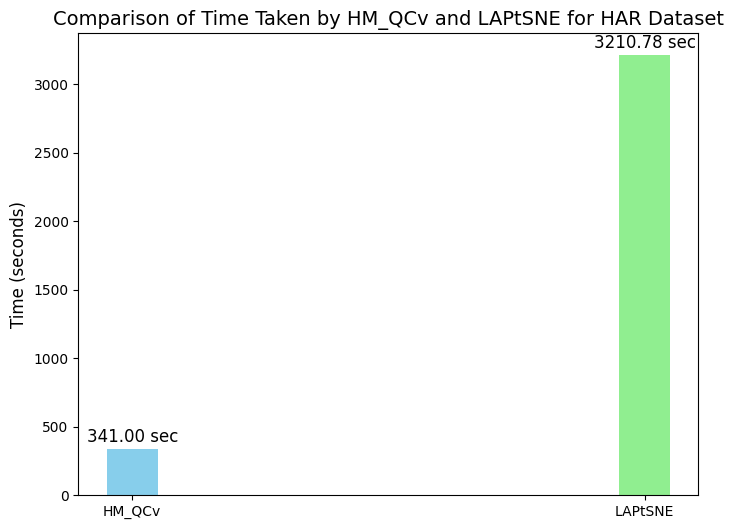
\includegraphics[width=0.95\textwidth]{HMQCvImages/HM_QCvvsLAPtSNE.png}  
    \caption{Comparison of Time Taken by proposed $HM\_QCv$ and existing LAPtSNE \cite{sun2023laplacian} for HAR \cite{har} Dataset}
    \label{hmqcvlaptsnecmp}
\end{figure}






Therefore, our approach, $HM\_QCv$, is more computationally efficient than LAPtSNE \cite{sun2023laplacian} and ensures local and global structure by preserving high-quality cluster visualization. This offers promising practical implications for data visualization.  


\subsection{Investigating Hyper-parameter sequences}




$HM\_QCv$ involves several tuning parameters (\textit{`$min\_dist$'}, \textit{`k'}, \textit{`NC'} and `\textit{$\lambda$}') that significantly affect the quality of cluster visualizations. The parameter \textit{`NC'} determines the number of clusters formed in the low-dimensional space. Setting \textit{`NC'} lower than the actual number of clusters can result in cluster overlap, while setting \textit{`NC'} higher may produce irrelevant or spurious clusters. For certain values of \textit{`k'}, reducing \textit{`$min\_dist$'} enhances cluster separation and improves metric scores. For certain values of \textit{`$min\_dist$'} and \textit{`k'}, increasing `\textit{$\lambda$}' further enhances the metric scores. Experiments are conducted with fixed values for \textit{`k'} and \textit{`NC'}, while varying the range of the parameters \textit{`$min\_dist$'} and `\textit{$\lambda$}'.  




Figure \ref{mindispar} examines reliable parameter values for \textit{`$min\_dist$'} on the HAR dataset using various metrics to optimize cluster visualization performance. A parameter sensitivity analysis was conducted, during which the neighbourhood parameter \textit{`k'} was fixed at 15 based on experimental results. The parameter \textit{`$min\_dist$'} was varied between 0.01 and 1, and the resulting values for three clustering metrics—NMI, SC, and DBI—were plotted to evaluate clustering quality across the specified range.


Analysis of Figure \ref{mindispar} reveals that the optimal value of \textit{`$min\_dist$'} is 0.15 , as both 
NMI and SC exhibit strong clustering structure and cohesion at this value.
\begin{itemize}
    \item The NMI (blue line) gradually increases as \textit{`$min\_dist$'} rises from 0.0 to 0.15, reflecting improved alignment between the clustering results and the ground truth. Beyond 0.15, NMI stabilizes, showing no significant gain or loss, which indicates consistent clustering quality within this range.
    \item The SC (green line) evaluates the cohesion and separation of clusters peaks near 0.15. Beyond this point, SC exhibits fluctuations with a general downward trend, suggesting that larger \textit{`$min\_dist$'} values may result in less compact and well-separated clusters. 
    \item Conversely, lower DBI (red line) values indicate better-defined clusters. As \textit{`$min\_dist$'} increases, DBI fluctuates, highlighting variations in the quality of cluster separation.
\end{itemize}



\begin{figure}[H]
    \centering
   
    \begin{minipage}{0.32\textwidth}
        \centering
        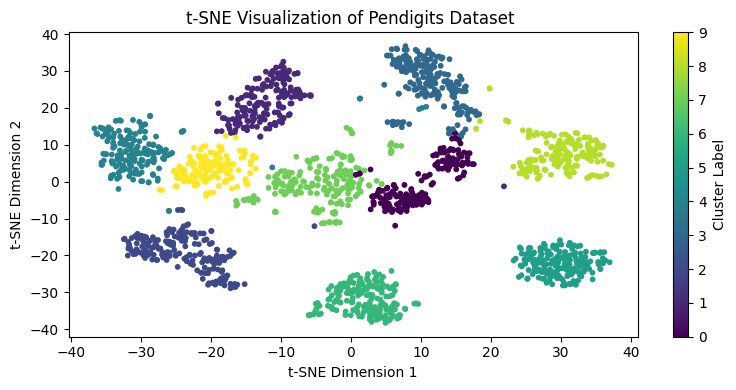
\includegraphics[width=0.95\textwidth]{HMQCvImages/tSNEonPendigits2.png}
        \caption*{\tiny{Pendigits - tSNE \cite{tsne}}}
    \end{minipage}
    \begin{minipage}{0.32\textwidth}
        \centering
        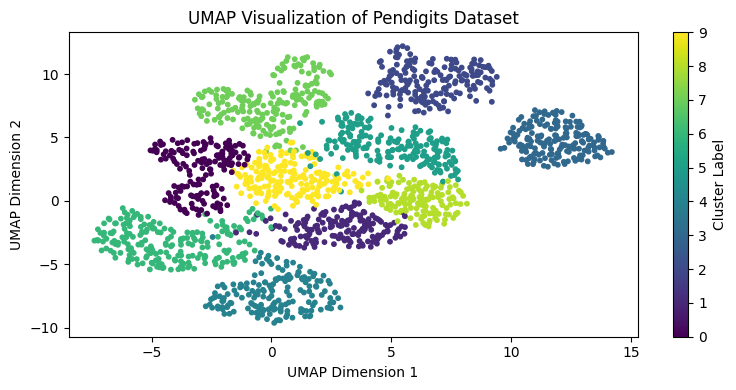
\includegraphics[width=0.95\textwidth]{HMQCvImages/UMAPonPendgits2.png}
        \caption*{\tiny{Pendigits - UMAP \cite{umap_reference}}}
    \end{minipage}
    \begin{minipage}{0.32\textwidth}
        \centering
        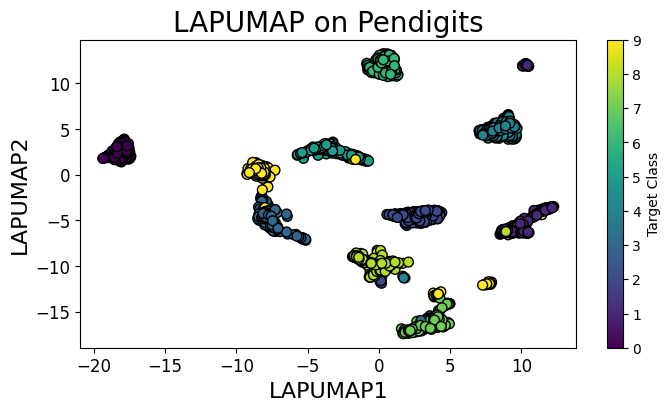
\includegraphics[width=0.95\textwidth]{HMQCvImages/LAPUMAP on Pendigits.png}
        \caption*{\tiny{Pendigits - $HM\_QCv$}}
    \end{minipage}
    %\begin{minipage}{0.24\textwidth}
        %\centering
        %\includegraphics[width=0.95\textwidth]{LAPtSNEPEN.png}
        %\caption*{\tiny{Pendigits - LAPtSNE}}
    %\end{minipage}



   
    \begin{minipage}{0.32\textwidth}
        \centering
        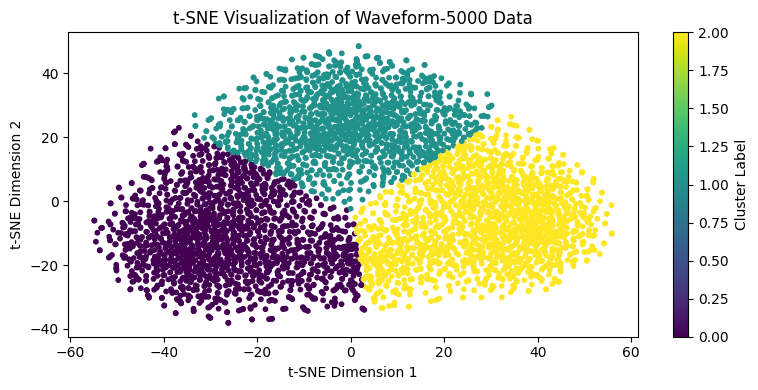
\includegraphics[width=0.95\textwidth]{HMQCvImages/tSNEonWaveform1.png}
        \caption*{\tiny{waveform - tSNE \cite{tsne}}}
    \end{minipage}
    \begin{minipage}{0.32\textwidth}
        \centering
        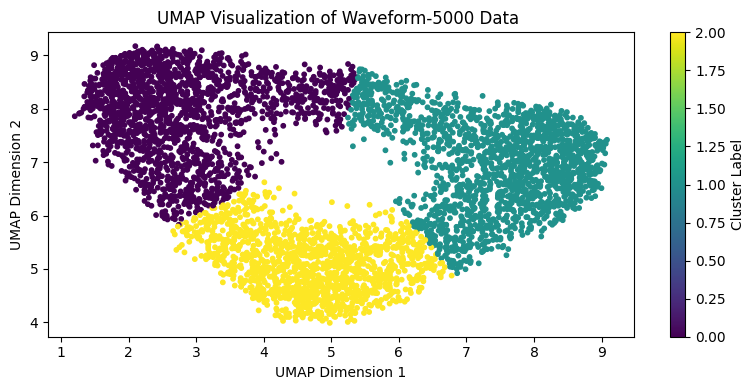
\includegraphics[width=0.95\textwidth]{HMQCvImages/UMAP on Waveform1.png}
        \caption*{\tiny{waveform - UMAP \cite{umap_reference}}}
    \end{minipage}
    \begin{minipage}{0.32\textwidth}
        \centering
        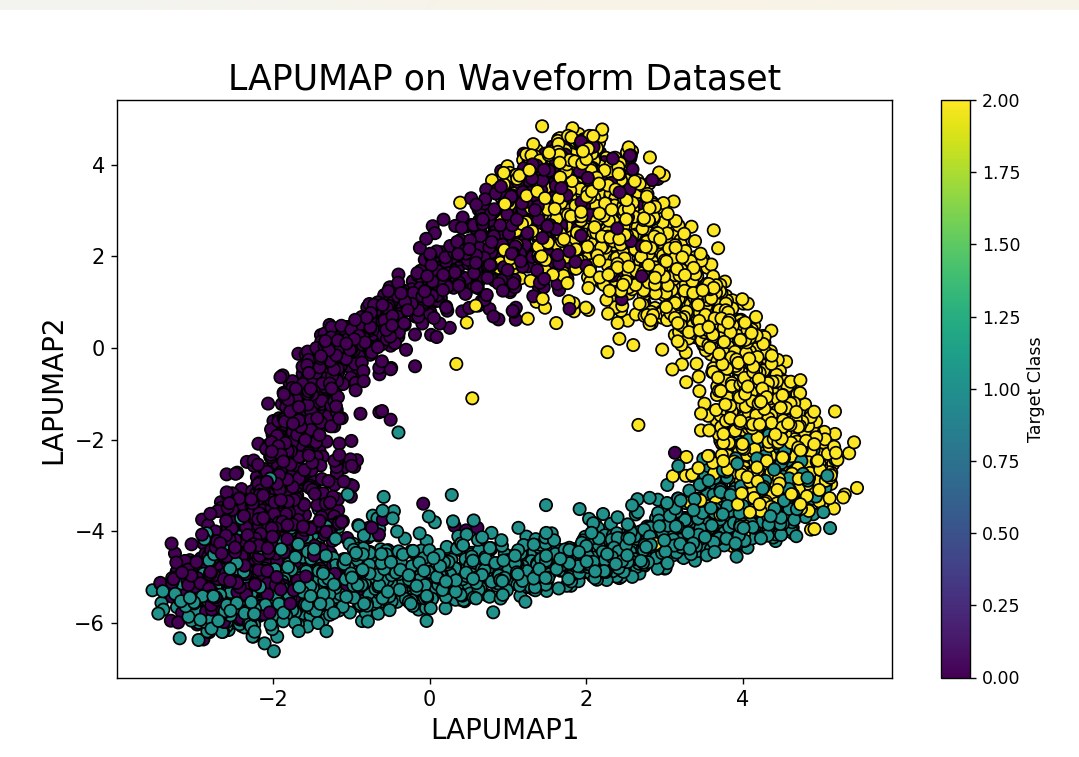
\includegraphics[width=0.95\textwidth]{HMQCvImages/LAPUMAP on WAVEFORM1.png}
        \caption*{\tiny{waveform - $HM\_QCv$}}
    \end{minipage}
    %\begin{minipage}{0.24\textwidth}
        %\centering
        %\includegraphics[width=0.95\textwidth]{LAPtSNEWAV.png}
        %\caption*{\tiny{waveform - LAPtSNE}}
    %\end{minipage}
 


   
    \begin{minipage}{0.32\textwidth}
        \centering
        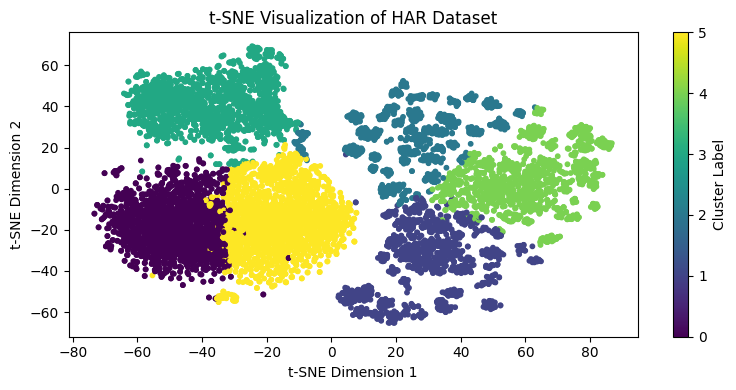
\includegraphics[width=0.95\textwidth]{HMQCvImages/HARtSNE.png}
        \caption*{\tiny{HAR - tSNE \cite{tsne}}}
    \end{minipage}
    \begin{minipage}{0.32\textwidth}
        \centering
        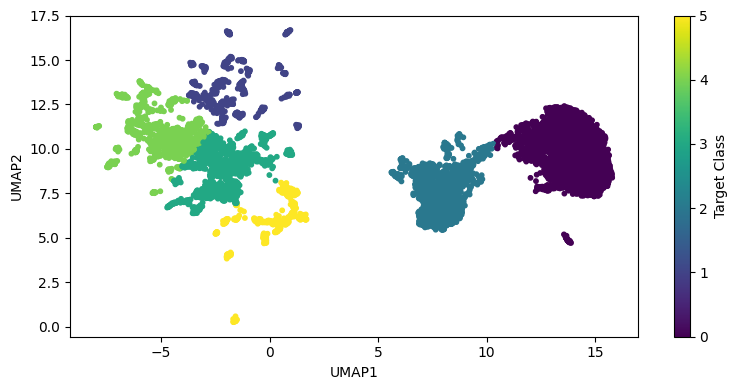
\includegraphics[width=0.95\textwidth]{HMQCvImages/HARUMAP.png}
        \caption*{\tiny{HAR - UMAP \cite{umap_reference}}}
    \end{minipage}
    \begin{minipage}{0.32\textwidth}
        \centering
        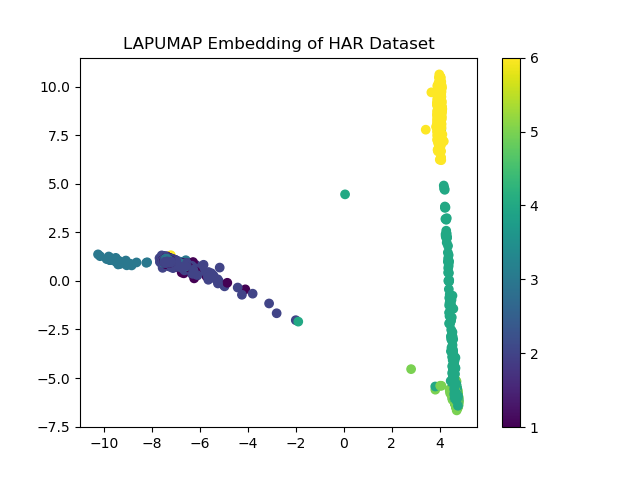
\includegraphics[width=0.95\textwidth]{HMQCvImages/HARGLUFINAL.png}
        \caption*{\tiny{HAR - $HM\_QCv$}}
    \end{minipage}
    %\begin{minipage}{0.24\textwidth}
       % \centering
        %\includegraphics[width=0.95\textwidth]{LAPtSNEHAR.png}
        %\caption*{\tiny{HAR - LAPtSNE}}
    %\end{minipage}



    \begin{minipage}{0.32\textwidth}
        \centering
        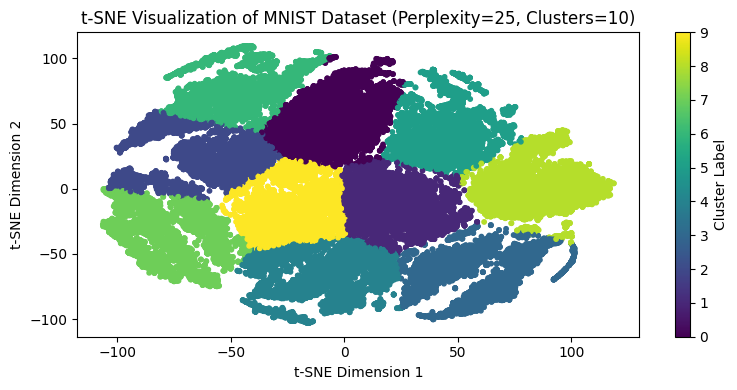
\includegraphics[width=0.95\textwidth]{HMQCvImages/MNISTtSNE.png}
        \caption*{\tiny{MNIST - tSNE \cite{tsne}}}
    \end{minipage}
    \begin{minipage}{0.32\textwidth}
        \centering
        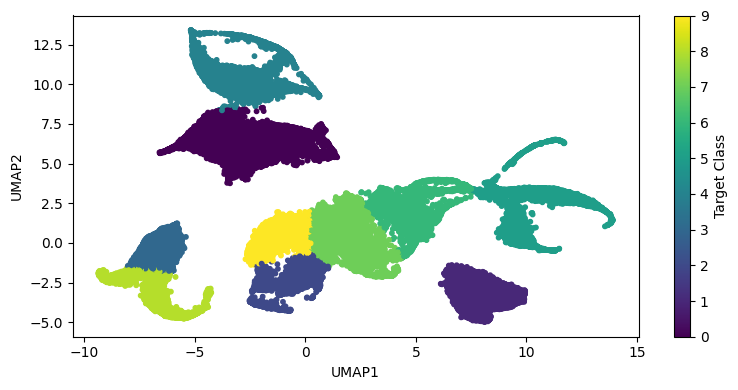
\includegraphics[width=0.95\textwidth]{HMQCvImages/MNISTUMAP.png}
        \caption*{\tiny{MNIST - UMAP \cite{umap_reference}}}
    \end{minipage}
    \begin{minipage}{0.32\textwidth}
        \centering
        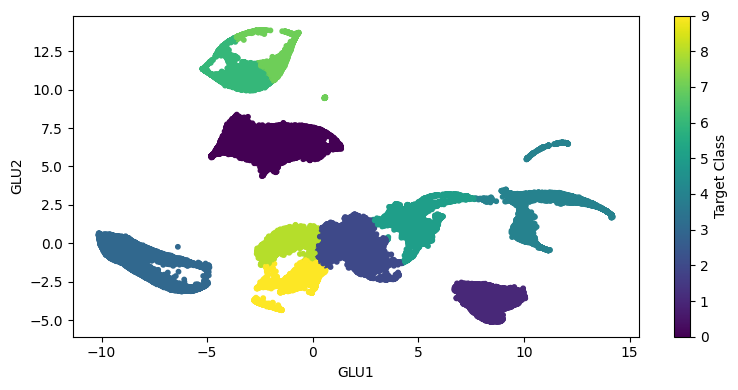
\includegraphics[width=0.95\textwidth]{HMQCvImages/MNISTGLUFINAL.png}
        \caption*{\tiny{MNIST - $HM\_QCv$}}
    \end{minipage}
    %\begin{minipage}{0.24\textwidth}
        %\centering
        %\includegraphics[width=0.95\textwidth]{LAPtSNEMNIST.png}
        %\caption*{\tiny{MNIST - LAPtSNE}}
    %\end{minipage}




    \begin{minipage}{0.32\textwidth}
        \centering
        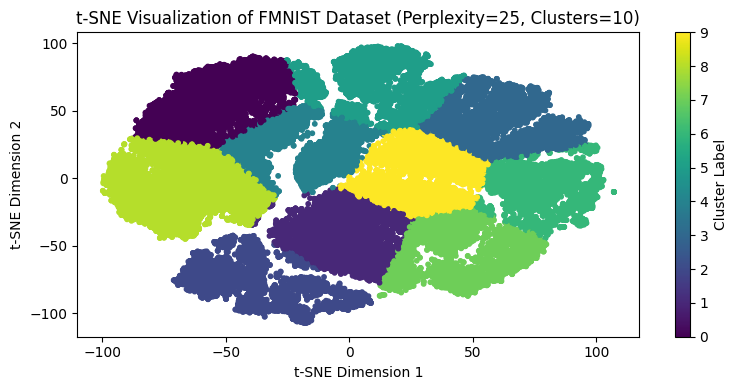
\includegraphics[width=0.95\textwidth]{HMQCvImages/FMNISTtSNE.png}
        \caption*{\tiny{FMNIST - tSNE \cite{tsne}}}
    \end{minipage}
    \begin{minipage}{0.32\textwidth}
        \centering
        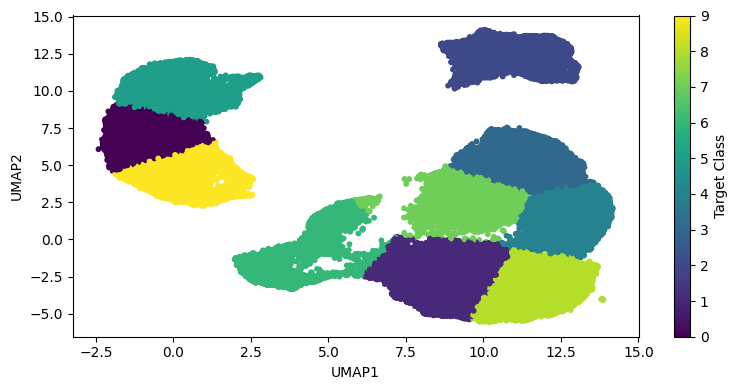
\includegraphics[width=0.95\textwidth]{HMQCvImages/FMNISTUMAP.png}
        \caption*{\tiny{FMNIST - UMAP \cite{umap_reference}}}
    \end{minipage}
    \begin{minipage}{0.32\textwidth}
        \centering
        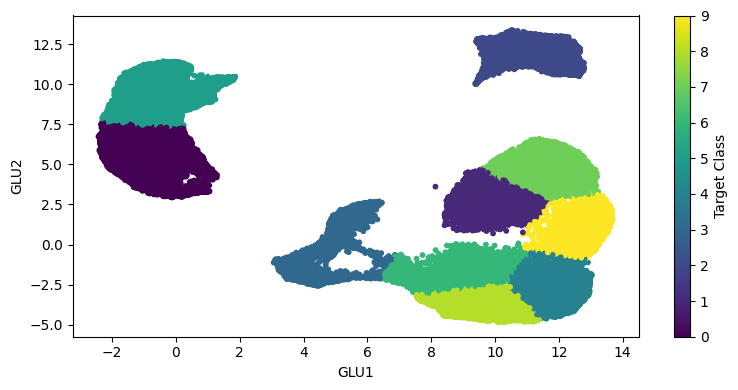
\includegraphics[width=0.95\textwidth]{HMQCvImages/HM_QCvFMNIST.png}
        \caption*{\tiny{FMNIST - $HM\_QCv$}}
    \end{minipage}
    %\begin{minipage}{0.24\textwidth}
        %\centering
        %\includegraphics[width=0.95\textwidth]{LAPtSNEFMNIST.png}
        %\caption*{\tiny{FMNIST - LAPtSNE}}
    %\end{minipage}



    \caption{Hybrid Model for Cluster Visualizations}
    \label{finalvizhmqcv}
\end{figure}






















This analysis indicates that \textit{`$min\_dist$'} value of 0.15 delivers the best clustering performance, characterized by high NMI ($\uparrow$), high SC ($\uparrow$), and low DBI ($\downarrow$) values. This combination demonstrates that the clusters are well-aligned with the ground truth, cohesive, and well-separated, making 0.15 a reliable choice for the optimal \textit{`$min\_dist$'} setting on the HAR dataset.


\begin{figure}[H]
    \centering
    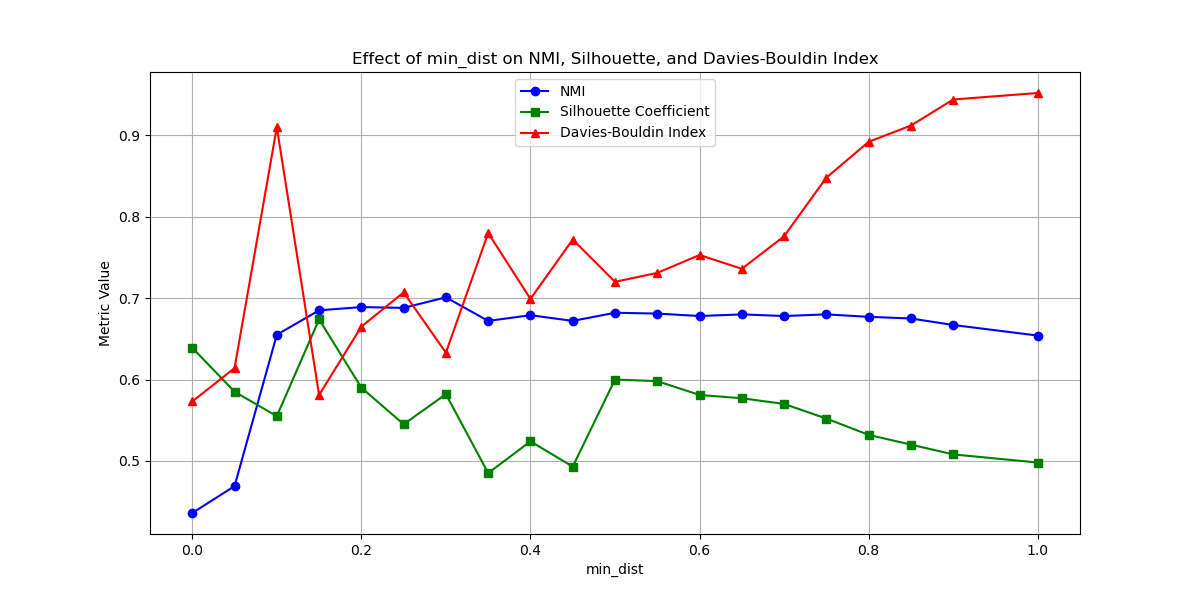
\includegraphics[width=0.95\textwidth]{HMQCvImages/Final_mindis.png}  
    \caption{Illustrating the consistency and robustness of the \textit{`$min\_dis$'} for HAR \cite{har} dataset with three different metrics.} 
    \label{mindispar}
\end{figure}

Figure \ref{lambdapar} presents the sensitivity analysis of the `\textit{$\lambda$}' parameter on the HAR dataset for cluster visualization performance, with \textit{`k'} fixed at 15, \textit{`$min\_dist$'} fixed at 0.15. This analysis explores the impact of varying `\textit{$\lambda$}' values within the range of 0.1 to 1.0 on three evaluation metrics: NMI, SC, and DBI. \\
Figure \ref{lambdapar} shows that changes in `\textit{$\lambda$}' have a distinct impact on each metric.


\begin{itemize}
    \item The NMI (blue line) remains relatively stable across varying `\textit{$\lambda$}' values, showing a slight upward trend. This consistency suggests that the clustering structure reliably aligns with the ground truth, even with moderate changes in `\textit{$\lambda$}' for this metric. Notably, the DBI is high at `\textit{$\lambda$}' = 1. 
    \item The SC (green line) gradually decreases from `\textit{$\lambda$}' = 0.1 to 0.3 and stabilizes at mid-range `\textit{$\lambda$}' values. As SC represents cluster cohesion and separation, it is observed that beyond `\textit{$\lambda$}' = 0.3, cluster cohesiveness shows no significant changes with further increases in `\textit{$\lambda$}'. However, at `\textit{$\lambda$}' = 1.0, there is a notable improvement.
    \item The DBI (red line) exhibits significant variations at `\textit{$\lambda$}' = 0.2, indicating poor cluster separation. However, DBI reaches its lowest value at `\textit{$\lambda$}' = 0.3, where the NMI and SC metrics stabilize, suggesting optimal cluster quality at this point. Beyond `\textit{$\lambda$}' = 0.3, DBI fluctuates, with a notable drop at `\textit{$\lambda$}' = 1.0, indicating sharp improvements in cluster separation quality at higher `\textit{$\lambda$}' values.
\end{itemize}


The results indicate that (\textit{$\lambda$} = 1.0, \textit{$min\_dist$} = 0.15 and \textit{k} = 15) deliver optimal cluster visualization performance, as assessed by the NMI, SC, and DBI metrics. These reliable parameter values effectively balance the trade-offs between alignment with the ground truth, cluster cohesion, and cluster separation, making them a robust parameter setting for visualizing clusters on the HAR dataset.



\begin{figure}[H]
    \centering
    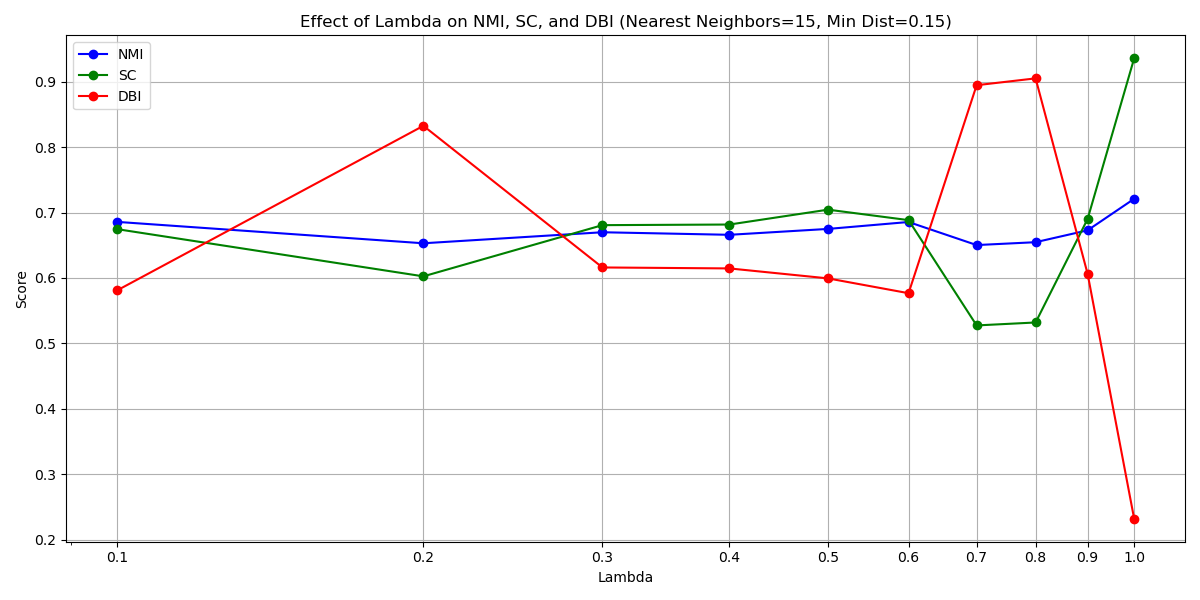
\includegraphics[width=0.95\textwidth]{HMQCvImages/Final_lambda.png}  
    \caption{Analysis of metric for determining the reliable regularization ($\lambda$) parameter value on HAR \cite{har} dataset.} %Sensitivity analysis for lambda on HAR \cite{har} dataset}
    \label{lambdapar}
\end{figure}



\subsection{Applications}


The proposed $HM\_QCv$ approach, an NLDR technique, finds wide application across various domains. This approach offers a unique perspective on complex datasets, analyzing and visualizing high-dimensional data while preserving meaningful local and global structures. It facilitates the identification of quality clusters, providing data insights for further analysis.

\begin{itemize}
    \item \textbf{Healthcare Analytics}\\
    The proposed approach $HM\_QCv$ is experimented with the HAR \cite{har} dataset shown in Section 4.5, where the cluster visualization helps to analyze the six activities of the patient.
    \item \textbf{ML Model Insights}\\
    The $HM\_QCv$ model is experimented with the Pendigits \cite{pendigits} and MNIST \cite{deng2012mnist} datasets, as shown in Sections 4.4 and 4.5. These experiments testify to the model's efficiency in visualizing digit classification through the importance of features in high-dimensional data. The additional experiment with the Waveform \cite{waveform} dataset shown in Section 4.4, which visualizes clusters in lower dimensions, further reinforces the model's efficiency in data visualization.
    \item \textbf{Exploratory Data Analysis (EDA)}\\
    The proposed approach, $HM\_QCv$, is experimented with the FMNIST \cite{fashionmnist} dataset shown in Section 4.5. This experiment establishes the model's reliability in exploratory data analysis. The cluster visualization helps to analyze similarities between different fashion categories. 

\end{itemize}

With the ability to handle complex and high-dimensional data, $HM\_QCv$ has a critical role in advancing research across diverse fields, offering researchers valuable methods to uncover and interpret hidden structures within data. Our proposed model is also apt for business analytics and time-series analysis applications.